\begin{frame}
  \frametitle{Measuring distance}
  %% \framesubtitle{}

  \begin{columns}[T]
    \begin{column}{60mm}
      \begin{itemize}
      \item \h{Distance} between vectors $\vu, \vv \in \setR^n$ \so
        (dis)\h{similarity}\\ of data points
        \begin{itemize}
        \item $\vu = (u_1, \ldots, u_n)$
        \item $\vv = (v_1, \ldots, v_n)$
        \end{itemize}
      \item \h{Euclidean} distance $\dist[2]{\vu}{\vv}$
      \item ``City block'' \h{Manhattan} distance $\dist[1]{\vu}{\vv}$
      \item Both are special cases of the \h{Minkowski} $p$-distance
        $\dist[p]{\vu}{\vv}$ (for $p\in [1, \infty]$)
      \end{itemize}
    \end{column}
    \begin{column}{40mm}
      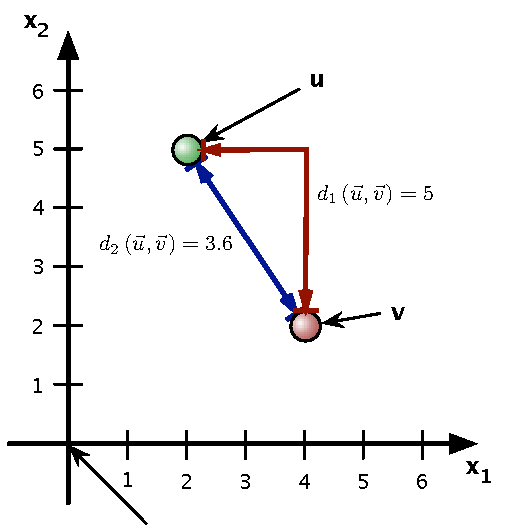
\includegraphics[width=40mm]{img/2_distance_examples}
    \end{column}
  \end{columns}
  \gap[.5]
    \[ \dist[p]{\vu}{\vv} \coloneq \bigl(
    \abs{u_1 - v_1}^p + \dots + \abs{u_n - v_n}^p
    \bigr)^{1/p} \] 
    %
    \[ \dist[\infty]{\vu}{\vv} = \max \bigset{\abs{u_1 - v_1}, \ldots, \abs{u_n - v_n}} \] 
\end{frame}

\begin{frame}
  \frametitle{Metric: a measure of distance}
  %% \framesubtitle{}

  \begin{itemize}
  \item A \h{metric} is a general measure of the distance $\dist{\vu}{\vv}$
    between points $\vu$ and $\vv$, which satisfies the following \h{axioms}:
    \begin{itemize}
      \item $\dist{\vu}{\vv} = \dist{\vv}{\vu}$
      \item $\dist{\vu}{\vv} > 0$ for $\vu \neq \vv$
      \item $\dist{\vu}{\vu} = 0$
      \item $\dist{\vu}{\vw} \leq \dist{\vu}{\vv} + \dist{\vv}{\vw}$
        (\h{triangle inequality})
    \end{itemize}
    \pause
  \item Metrics form a very broad class of distance measures, some of which do
    not fit in well with our geometric intuitions%
    \pause
  \item E.g., metric need not be \h{translation-invariant}
    \[ \dist{\vu+\vx}{\vv+\vx} \neq \dist{\vu}{\vv} \]
    \pause\ungap
  \item Another unintuitive example is the \hh{discrete metric}
    \[
    \dist{\vu}{\vv} =
    \begin{cases}
      0 & \vu = \vv \\
      1 & \vu \neq \vv
    \end{cases}
    \]
  \end{itemize}
\end{frame}

%%% Local Variables: 
%%% mode: latex
%%% TeX-master: "../../workspace"
%%% End: 
